The content-based part of the algorithm starts like the collaborative part by generating coefficients, but this time for media items instead of users. This is done by comparing vectors which each media and user has, that indicates whether or not they have a certain property for media, and preferences for users. These properties is currently genre and which associated people is connected to the vector. For the media, the vector is simply be boolean 0 and 1, indicating whether or not they have something, while the user vector can be higher, lower, and decimals which is altered by personal preferences. An associated person can be an actor for a movie, or an author for a book.

\subsubsection{Vectors}

These vectors is dynamically updated, as new associated people enters the system. The genre part of the vector is static, and corresponds to the predefined genres available in the system. When a new associated person is being created in the system, the users' vectors is updated to accommodate this. This means that the user will always have a vector with the same length as the media with the most recently added associated person. See Figure \ref{VectorUpdate} for an example.

\begin{figure}[htb]
\centering
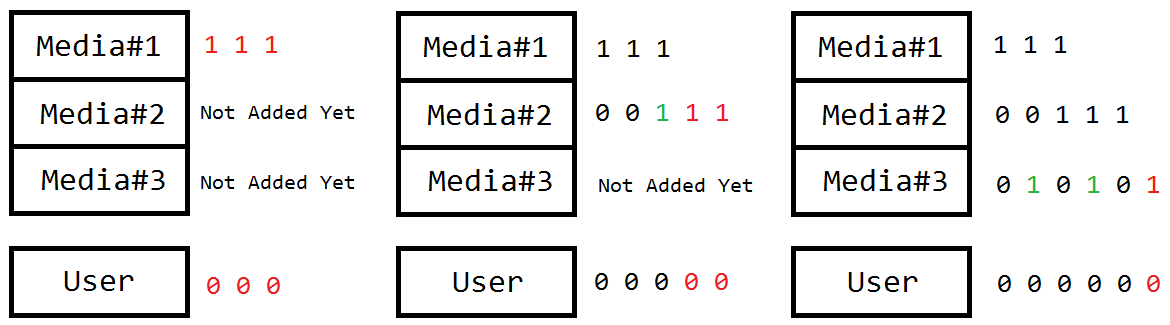
\includegraphics[width=0.8\textwidth]{Images/VectorUpdate.png}
\caption{Vector updates as new media is added}
\label{VectorUpdate}
\end{figure}

Each media is added to the collection one by one, with each addition all users in the system is updated as it is required. Red numbers indicate that the certain person was not already part of the vectors, and therefore had to be added to all the user vectors, and the certain media itself. Green numbers indicate the person already have a spot in the vectors, and therefore did not have to update all the user vectors.

Users can change their vectors by adding media to their medialists. This process will convert the rating the user gave into a number, using the method seen in Listing \ref{ConvertRating}.

\begin{lstlisting}[caption={The CompareUserPair method of the recommendation algorithm},label={ConvertRating}]
private double ConvertRating(double rating)
{
	return (rating / 5) - 1;
}
\end{lstlisting}

The user can give a rating in the range of 0 til 10. The method will then return a number between -1 and 1, where -1 is 0 and 1 is 10. This number will then be added to the user vector in each corresponding spot where the added media has a 1. For an example, see Table \ref{AddMediaEx}.

\begin{table}[htb]
\centering
\begin{tabular}{|l|l|l|l|l|l|l|l|} \hline
	\textbf{Media} & \textbf{Rating} & \textbf{0} & \textbf{1} & \textbf{2} & \textbf{3} & \textbf{4} & \textbf{5} \\ \hline
	Media 3 & 7 & 0 & 0.4 & 0 & 0.4 & 0 & 0.4 \\ \hline
	Media 2 & 2 & 0 & 0.4 & -0.6 & -0.2 & -0.6 & 0.4 \\ \hline
\end{tabular}
\caption{User vector alteration upon adding media to their medialist}
\label{AddMediaEx}
\end{table}

When a user adds media 3 and 2 which can be seen in Figure \ref{VectorUpdate}, and gives them a rating of 7 and 2, respectively. The 7 is converted into 0.4, and is added to the user vector corresponding to the media vector. The same happens with the other media, except it is a negative number. This is the result of a user giving a media item a low rating. The user vector should then be a representation of what he likes and dislikes.

\subsubsection{Vector Comparison}

By comparing the vectors, you can generate a coefficient for how well a certain media suits the taste of a user. If the media hits a lot of the positive spots in the user vector, it will receive a high coefficient. Of course, it can also receive a low, or even a negative coefficient, if it hits negative spots in the user vector. See Table \ref{ContentEx} for an example using the previous user and media examples.

\begin{table}[htb]
\centering
\begin{tabular}{|l|l|l|l|l|l|l|} \hline
	\textbf{User} & 0 & 0.4 & -0.6 & -0.2 & -0.6 & 0.4 \\ \hline
	\textbf{Media 1} & 1 & 1 & 1 & 0 & 0 & 0 \\ \hline
	\textbf{Media 4} & 1 & 1 & 0 & 0 & 0 & 1 \\ \hline
\end{tabular}
\caption{Content Example}
\label{ContentEx}
\end{table}

The comparison is done by using the cosine distance as described in Section \ref{ContentBasedDes}, and returns $-0.062$ for the first media item and $0.247$ for the second media item. During the content-based algorithm, every media the user have not already consumed, is assigned a coefficient through this method. The algorithm will then sort and choose the media with the highest coefficients, and returns them as its recommended media. See Listing \ref{CompareVector} for the part of the algorithm which calculates this coefficient.

\begin{lstlisting}[caption={The CompareVectorRepresentations method},label={CompareVector}]
private double CompareVectorRepresentations(List<double> userRepresentation, List<bool> mediaRepresentation, double userLength, double mediaLength)
{
	double commonPoints = 0;

	for (int i = 0; i < mediaRepresentation.Count; i++)
	{
		if (userRepresentation[i] != 0 && mediaRepresentation[i])
		{
			commonPoints += userRepresentation[i];
		}
	}

	if (commonPoints == 0)
		return 0;

	return FindCosineDistance(commonPoints, userLength, mediaLength);
}
\end{lstlisting}

The media vector is actually a list of booleans, rather than a list of doubles, like the user vector is. The loop will run for the length of the media vector, and will ignore anything past that point in the user vector, since it cannot hit any more common points. If any common points were found, the function will return the result of the cosine distance calculation. The lengths were determined prior to the call of the compare functions, and were passed as parameters.